\section{量子统计中的分布函数}


\begin{quotation}
``计算的途径有两种。第一种,是我所愿意采用的,是先有一幅清晰的物理图象。第二种是严格的数学架构。''\qquad 费米
\end{quotation}




假设一个量子力学系统,由N($ \sim 10^{23} $,宏观系统)个全同粒子组成,
系统能量本征值为$\varepsilon _i $,相应能级简并度为$g_i $,假设有$n_i$个粒子占据能级$\varepsilon _i $,则:$\sum\limits_i {n_i }  = N$,$\sum\limits_i {n_i \varepsilon _i }  = E$。
假设总粒子数N固定,总能量E也固定,即系统与外界无粒子与能量的交换。

根据泡利原理,一个量子态只能被一个费米子占据;而对玻色子而言,一个量子态可被不限个数的玻色子所占据。


\subsection{粒子在能级$\varepsilon _i $上的分布}

考虑能级$\varepsilon _i $,能级简并度为$g_i $

对费米子而言,由于一个状态上最多只能占据一个费米子,所以相当于在$g_i$个抽屉内放$n_i$个相同的球,
并且每个抽屉内最多只能放1个球。对应的方式数就是从$g_i$个抽屉中挑选出$n_i$个抽屉的组合数$\left( {\begin{array}{*{20}c}
   {g_i }  \\
   {n_i }  \\
\end{array}} \right)$,
所以$n_i$个费米子占据$g_i$个状态的方式数为:


\begin{equation}\label{33-1}
\Omega _i^{FD}  = \frac{{g_i !}}{{n_i !\left( {g_i  - n_i } \right)!}}
\end{equation}

对玻色子而言,由于一个状态上可以占据多个玻色子,所以相当于向$g_i$个抽屉内放$n_i$个相同的球,
并且不限制每个抽屉内球的个数。可以把抽屉的两壁档板想象为白球,玻色子看为黑球,
由于最两端抽屉外侧档板永远为白球,不影响方式数,所以可以不考率。
这样问题就转化为$\left( {g_i  - 1} \right)$个白球与$n_i$个黑球的组合问题,组合数为:$\left( {\begin{array}{*{20}c}
   {g_i  + n_i  - 1}  \\
   {n_i }  \\
\end{array}} \right)$,
所以$n_i$个玻色子占据$g_i$个状态的方式数:

\begin{equation}\label{33-2}
\Omega _i^{BE}  = \frac{{\left( {g_i  + n_i  - 1} \right)!}}{{n_i !\left( {g_i  - 1} \right)!}}
\end{equation}


考虑经典粒子,由于经典粒子可以分辨,并可占据相同状态,所以每个粒子都有$g_i$种可能,总的方式数为$g_i ^{n_i } $。
$n_i$个经典粒子(可分辨粒子)占据$g_i$个状态的方式数:

\begin{equation}\label{33-3}
\Omega _i^{BM}  = g_i ^{n_i }
\end{equation}


\subsection{粒子的最可几分布}


假设粒子数在各能级上的分布为:$\left\{ {n_i } \right\} = \left\{ {n_1 ,n_2 ,n_3 ,...} \right\}$,$\sum\limits_i {n_i }  = N$

N个费米子处于分布$\left\{ {n_i } \right\}$的方式数为:

\begin{equation}\label{33-4}
\Omega _{\left\{ {n_i } \right\}}^{FD}  = \prod\limits_i {\Omega _i^{FD} }  = \prod\limits_i {\frac{{g_i !}}{{n_i !\left( {g_i  - n_i } \right)!}}}
\end{equation}


N个玻色子处于分布$\left\{ {n_i } \right\}$的方式数为:


\begin{equation}\label{33-5}
\Omega _{\left\{ {n_i } \right\}}^{BE}  = \prod\limits_i {\Omega _i^{BE} }  = \prod\limits_i {\frac{{\left( {g_i  + n_i  - 1} \right)!}}{{n_i !\left( {g_i  - 1} \right)!}}}
\end{equation}

N个经典粒子处于分布$\left\{ {n_i } \right\}$的方式数为\footnote{考虑到经典粒子是可以辨别的,
所以不同能级间每交换一次粒子,都对应一个新的分布,
相同能级内交换粒子导致新的分布由于在计算$\Omega _i^{BE} $时已经考虑过,所以在这里就不必重复计算了,所以这里需要乘以因子$\frac{{N!}}{{\prod\limits_i {n_i !} }}$}:

\begin{equation}\label{33-6}
\Omega _{\left\{ {n_i } \right\}}^{BM}  = \frac{{N!}}{{\prod\limits_i {n_i !} }}\prod\limits_i {\Omega _i^{BE} }  = N!\prod\limits_i {\frac{{g_i ^{n_i } }}{{n_i !}}}
\end{equation}

\subsubsection{费米-狄拉克统计}

\index{Fermi-Dirac statistics: 费米-狄拉克统计}

最可几分布条件:分布$\left\{ {n_i } \right\}$的方式数取最大值,根据等几率原理,相应分布$\left\{ {n_i } \right\}$的几率最大,此时应满足变分为0的条件:$\delta \Omega _{\left\{ {n_i } \right\}}^{FD}  = 0$,为计算简便,我们取变分条件为:$\delta \ln \Omega _{\left\{ {n_i } \right\}}^{FD}  = 0$

根据$\sum\limits_i {n_i }  = N$,$\sum\limits_i {n_i \varepsilon _i }  = E$,有:$\delta N = \delta \sum\limits_i {n_i }  = 0$,$\delta E = \delta \sum\limits_i {\varepsilon _i n_i }  = 0$

所以:

$\begin{array}{l}
 \delta \left[ {\ln \Omega _{\left\{ {n_i } \right\}}^{FD}  - \alpha \sum\limits_i {n_i }  - \beta \sum\limits_i {\varepsilon _i n_i } } \right] = \delta \left[ {\sum\limits_i {\ln \Omega _i^{FD} }  - \alpha \sum\limits_i {n_i }  - \beta \sum\limits_i {\varepsilon _i n_i } } \right] \\
  = \sum\limits_i {\delta n_i \left[ {\frac{{\partial \ln \Omega _i^{FD} }}{{\partial n_i }} - \alpha  - \beta \varepsilon _i } \right]}  = 0 \\
 \end{array}$


$\ln \Omega _i^{FD}  = \ln \frac{{g_i !}}{{n_i !\left( {g_i  - n_i } \right)!}} = \ln g_i ! - \ln n_i ! - \ln \left( {g_i  - n_i } \right)!$



假设$g_i  \gg n_i  \gg 1$,利用斯特林近似\footnote{斯特林近似:$\ln n! = \ln 1 + \ln 2 + ... + \ln n$,当$n \to \infty $时,$\ln n! \approx \mathop {\lim }\limits_{x = n \to \infty } \int_1^x {\ln xdx} $

即:$\ln x! = \int_1^x {\ln xdx}  = \left[ {x\ln x} \right]_1^x  - \int_1^x {xd\ln x}  = x\ln x - \int_1^x {dx}  = x\ln x - x + 1$

所以:当$x \to \infty $,$\ln x! = x\ln x - x$}:


$\begin{array}{l}
 \ln \Omega _i^{FD}  = \ln \frac{{g_i !}}{{n_i !\left( {g_i  - n_i } \right)!}} = \ln g_i ! - \ln n_i ! - \ln \left( {g_i  - n_i } \right)! \\
  \approx g_i \ln g_i  - g_i  - n_i \ln n_i  + n_i  - \left( {g_i  - n_i } \right)\ln \left( {g_i  - n_i } \right) + \left( {g_i  - n_i } \right) \\
  = g_i \ln g_i  - n_i \ln n_i  - \left( {g_i  - n_i } \right)\ln \left( {g_i  - n_i } \right) \\
 \end{array}$


$\begin{array}{l}
 \frac{{\partial \ln \Omega _i^{FD} }}{{\partial n_i }} = \frac{\partial }{{\partial n_i }}\left[ {g_i \ln g_i  - n_i \ln n_i  - \left( {g_i  - n_i } \right)\ln \left( {g_i  - n_i } \right)} \right] \\
  =  - \left[ {\ln n_i  + 1 - \ln \left( {g_i  - n_i } \right) - 1} \right] = \left[ {\ln \left( {g_i  - n_i } \right) - \ln n_i } \right] = \ln \frac{{g_i  - n_i }}{{n_i }} \\
 \end{array}$


所以:

$ \delta \left[ {\ln \Omega _{\left\{ {n_i } \right\}}^{FD}  - \alpha \sum\limits_i {n_i }  - \beta \sum\limits_i {\varepsilon _i n_i } } \right]  =  \sum\limits_i {\delta n_i \left[ {\ln \frac{{g_i  - n_i }}{{n_i }} - \alpha  - \beta \varepsilon _i } \right]}  = 0$.

即:$\left[ {\ln \frac{{g_i  - n_i }}{{n_i }} - \alpha  - \beta \varepsilon _i } \right] = 0$,所以:$\ln \frac{{g_i  - n_i }}{{n_i }} = \alpha  + \beta \varepsilon _i $,$\frac{{g_i  - n_i }}{{n_i }} = \frac{{g_i }}{{n_i }} - 1 = \exp \left[ {\alpha  + \beta \varepsilon _i } \right]$


所以:$\left\langle {n_i } \right\rangle _{FD}  = \frac{{g_i }}{{\exp \left( {\alpha  + \beta \varepsilon _i } \right) + 1}}$,定义:$\beta  = \frac{1}{{k_B T}}$,$\alpha  =  - \frac{\mu }{{k_B T}} =  - \mu \beta $

得到费米-狄拉克统计:


\begin{equation}\label{33-7}
\left\langle {n_i } \right\rangle _{FD}  = \frac{{g_i }}{{\exp \left( {{\textstyle{{\varepsilon _i  - \mu } \over {k_B T}}}} \right) + 1}}
\end{equation}


\subsubsection{玻色-爱因斯坦统计}

\index{Bose-Einstein statistics: 玻色-爱因斯坦统计}

$\begin{array}{l}
 \ln \Omega _i^{BE}  = \ln \frac{{\left( {g_i  + n_i  - 1} \right)!}}{{n_i !\left( {g_i  - 1} \right)!}} = \ln \left( {g_i  + n_i  - 1} \right)! - \ln n_i ! - \ln \left( {g_i  - 1} \right)! \\
  \approx \left( {g_i  + n_i  - 1} \right)\ln \left( {g_i  + n_i  - 1} \right) - n_i \ln n_i  - \left( {g_i  - 1} \right)\ln \left( {g_i  - 1} \right) \\
 \end{array}$


$\begin{array}{l}
 \frac{{\partial \ln \Omega _i^{BE} }}{{\partial n_i }} = \frac{\partial }{{\partial n_i }}\left[ {\left( {g_i  + n_i  - 1} \right)\ln \left( {g_i  + n_i  - 1} \right) - n_i \ln n_i  - \left( {g_i  - 1} \right)\ln \left( {g_i  - 1} \right)} \right] \\
  = \ln \left( {g_i  + n_i  - 1} \right) - \ln n_i  = \ln \frac{{g_i  + n_i  - 1}}{{n_i }} \\
 \end{array}$


$\ln \frac{{g_i  + n_i  - 1}}{{n_i }} = \alpha  + \beta \varepsilon _i $, 所以:$\frac{{g_i  + n_i  - 1}}{{n_i }} \approx \frac{{g_i  + n_i }}{{n_i }} = \exp \left[ {\alpha  + \beta \varepsilon _i } \right]$
($g_i  \gg n_i  \gg 1$)


得到玻色-爱因斯坦统计:

\begin{equation}\label{33-8}
\left\langle {n_i } \right\rangle _{BE}  = \frac{{g_i }}{{\exp \left( {\alpha  + \beta \varepsilon _i } \right) - 1}} = \frac{{g_i }}{{\exp \left( {{\textstyle{{\varepsilon _i  - \mu } \over {k_B T}}}} \right) - 1}}
\end{equation}




\subsubsection{玻尔兹曼-麦克斯韦统计}

\index{Boltzmann-Maxwell statistics: 玻尔兹曼-麦克斯韦统计}

$\ln \Omega _{\left\{ {n_i } \right\}}^{BM}  = \ln N!\prod\limits_i {\frac{{g_i ^{n_i } }}{{n_i !}}}  = \ln N! + \sum\limits_i {\ln \frac{{g_i ^{n_i } }}{{n_i !}}} $

$\begin{array}{l}
 \delta \left[ {\ln \Omega _{\left\{ {n_i } \right\}}^{BM}  - \alpha \sum\limits_i {n_i }  - \beta \sum\limits_i {\varepsilon _i n_i } } \right] = \delta \left[ {\ln N! + \sum\limits_i {\ln \frac{{g_i ^{n_i } }}{{n_i !}}}  - \alpha \sum\limits_i {n_i }  - \beta \sum\limits_i {\varepsilon _i n_i } } \right] \\
  = \sum\limits_i {\delta n_i \left[ {\frac{\partial }{{\partial n_i }}\left( {\ln \frac{{g_i ^{n_i } }}{{n_i !}}} \right) - \alpha  - \beta \varepsilon _i } \right]}  = 0 \\
 \end{array}$

$\ln \frac{{g_i ^{n_i } }}{{n_i !}} = n_i \ln g_i  - \ln n_i ! \approx n_i \ln g_i  - n_i \ln n_i  + n_i $

所以:$\frac{\partial }{{\partial n_i }}\left( {\ln \frac{{g_i ^{n_i } }}{{n_i !}}} \right) = \frac{\partial }{{\partial n_i }}\left( {n_i \ln g_i  - n_i \ln n_i  + n_i } \right) = \ln g_i  - \ln n_i  = \ln \frac{{g_i }}{{n_i }}$

$\ln \frac{{g_i }}{{n_i }} = \alpha  + \beta \varepsilon _i $,得到玻尔兹曼-麦克斯韦统计:


\begin{equation}\label{33-9}
\left\langle {n_i } \right\rangle _{BM}  = \frac{{g_i }}{{\exp \left[ {\alpha  + \beta \varepsilon _i } \right]}} = \frac{{g_i }}{{\exp \left[ {{\textstyle{{\varepsilon _i  - \mu } \over {k_B T}}}} \right]}}
\end{equation}


\subsection{费米气体}

\index{Fermi gas: 费米气体}

考虑无相互作用费米子的集合,

$N = \sum\limits_i {\left\langle {n_i } \right\rangle _{FD} }  = \sum\limits_i {\frac{{g_i }}{{\exp \left( {{\textstyle{{\varepsilon _i  - \mu } \over {k_B T}}}} \right) + 1}}} $

如果能级很密,可以把求和换为积分;


$N = \int_0^\infty  {f\left( \varepsilon  \right)D\left( \varepsilon  \right)d\varepsilon } $


其中:$f\left( \varepsilon  \right) = \frac{1}{{\exp \left( {{\textstyle{{\varepsilon  - \mu } \over {k_B T}}}} \right) + 1}}$,$D\left( \varepsilon  \right) = \frac{{dg}}{{d\varepsilon }}$为态密度。


$\mathop {\lim }\limits_{T \to 0} f\left( \varepsilon  \right) = \left\{ \begin{array}{l}
 0,\varepsilon  > \mu  \\
 {\textstyle{1 \over 2}},\varepsilon  = \mu  \\
 1,\varepsilon  < \mu  \\
 \end{array} \right.$


\begin{figure}[h]
\begin{center}
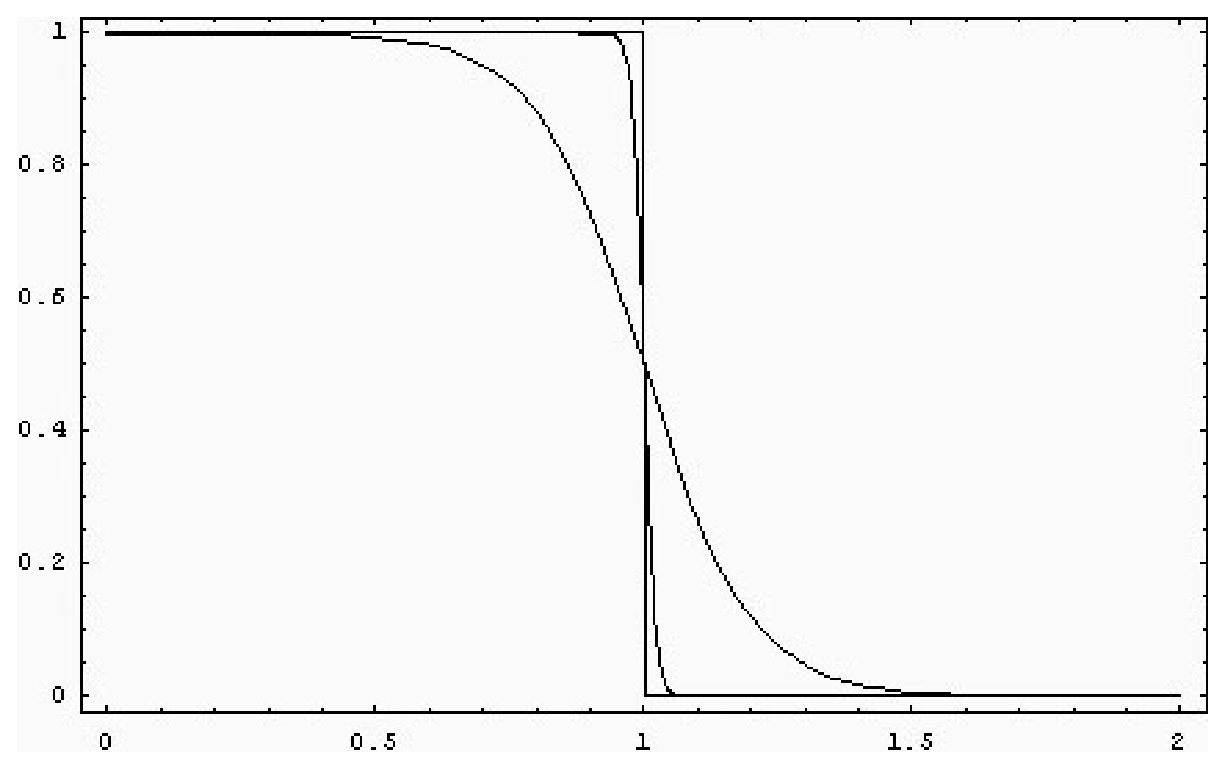
\includegraphics[clip,width=7cm]{IdenticalParticles/33-1.ps}
\caption{不同温度下费米-狄拉克分布函数$f(\varepsilon)$}
\end{center}
\end{figure}

费米气体在$T \to 0$(基态)时,最多填充到$\varepsilon  = \mu $处,这个数值叫费米能$\varepsilon _F $。
无相互作用费米子能量可表示为:$\varepsilon  = \frac{{\hbar ^2 k^2 }}{{2m}}$;动量空间中,费米气体基态是以$k_F  = \frac{{\sqrt {2m\varepsilon _F } }}{\hbar }$为半径的球体,半径$k_F$所张成球面称为费米面。当$T \ne 0$时,根据分布函数$f\left( \varepsilon  \right) = \frac{1}{{\exp \left( {{\textstyle{{\varepsilon  - \mu } \over {k_B T}}}} \right) + 1}}$知道,费米面附近$\Delta \varepsilon  \sim k_B T$的费米子将偏离满占据,从而出现``空穴'',因此只有$k_B T$壳层附近的电子才会对跃迁过程有贡献。


\subsection{费米液体}

\index{Fermi liquid: 费米液体}

\begin{figure}[h]
\begin{center}
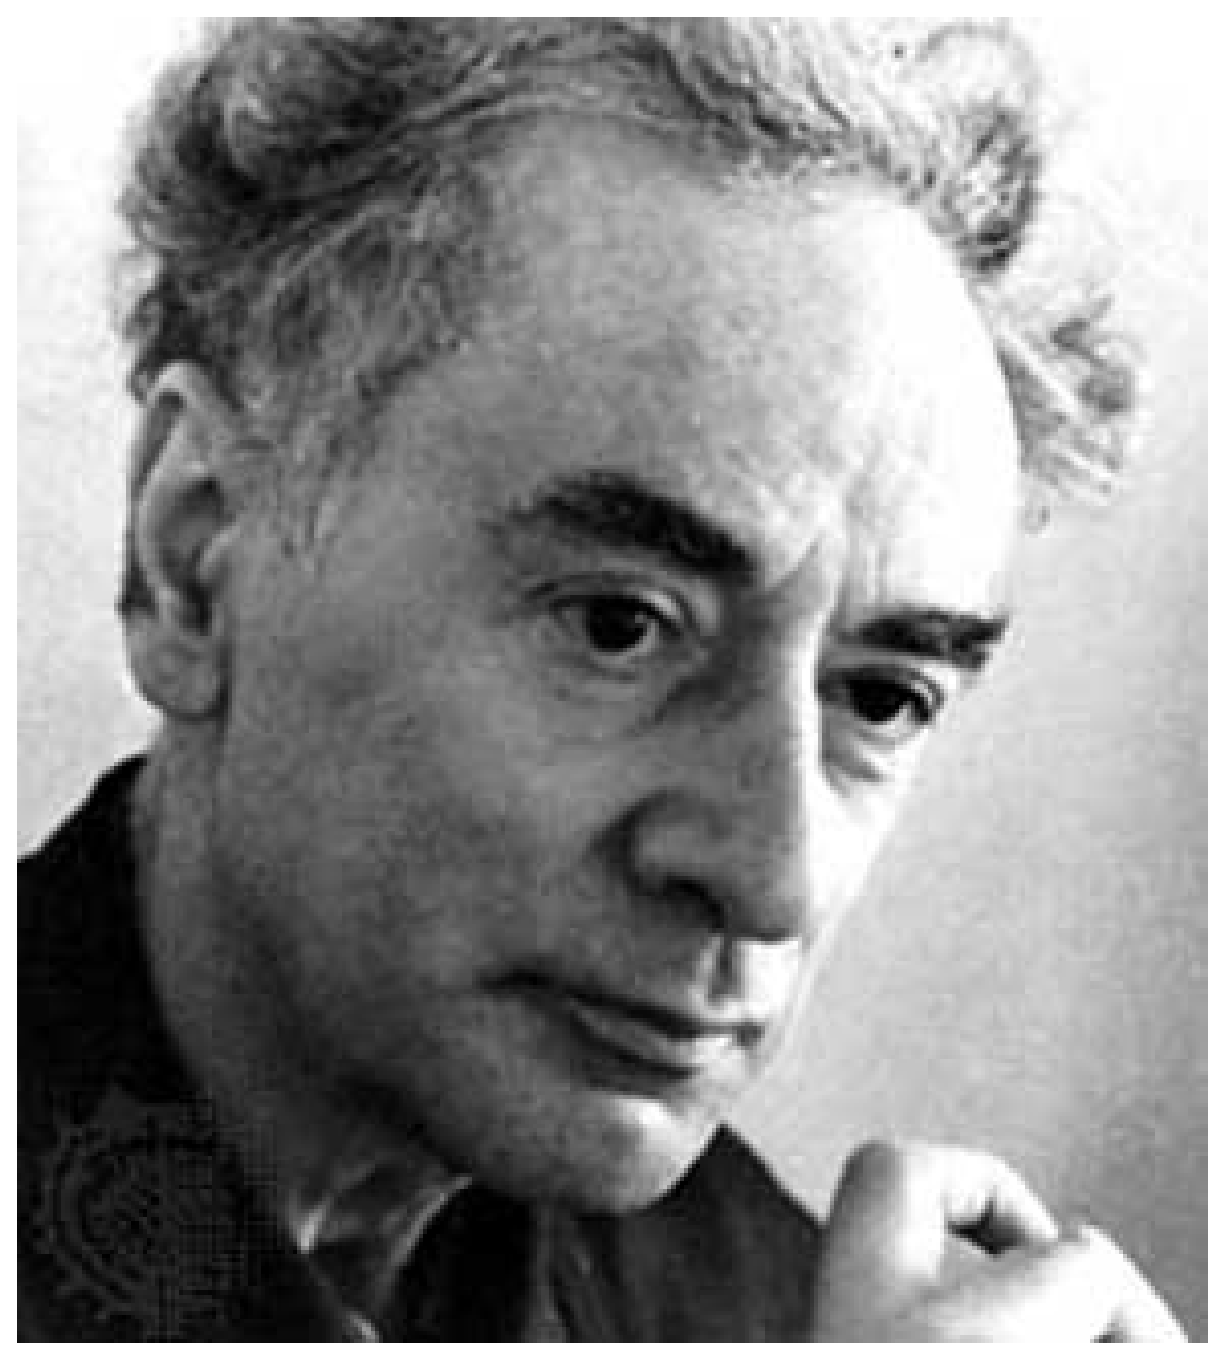
\includegraphics[clip,width=6cm]{IdenticalParticles/landau.ps}
\caption{朗道}
\end{center}
\end{figure}


如果在无相互作用费米子(电子)之间引入弱的相互作用,使原有系统能级不发生本质性改变;
我们将得到所谓的费米液体\footnote{参考朗道《统计物理学 II》第1章}。
在费米液体中,由于费米子间存在不可忽略的相互作用,我们无法把单个费米子的运动从系统整体运动中分离开来,
独立粒子的图象不再严格适用,费米子能量无法表示为$\varepsilon  = \frac{{\hbar ^2 k^2 }}{{2m}}$的形式。
但由于系统能级未发生本质性改变,独立粒子的图象仍近似成立,为区别于严格意义上的独立粒子,我们称之为准粒子。
费米液体可以使用准粒子概念进行描述,准粒子之间可看作是``无相互作用''的,准粒子数目与系统中原有费米子数目相等。
准粒子可认为是在所有费米子的平均场中运动的粒子,因此仍具有确定能量$\varepsilon $和动量p,
但粒子的有效质量将发生改变$\varepsilon  = \frac{{\hbar ^2 k^2 }}{{2m^* }}$,同时准粒子的寿命$\tau$也将发生改变。

\index{Quasiparticle: 准粒子}

\textbf{准粒子图象适用的物理条件:}
准粒子图象下,费米面概念仍然有效,为保证费米面的``清晰性''和``稳定性'',
准粒子能量的不确定度应远小于热涨落能量:$\delta \varepsilon  \sim \frac{\hbar }{\tau } \ll k_B T$;

其中$\tau$:准粒子寿命,应反比于准粒子的跃迁速率。跃迁速率正比于跃迁过程末态的数目($ \propto k_B T$),同时也正比于跃迁过程初态的数目($ \propto k_B T$)。所以:$\frac{1}{\tau } \sim A \sim \left( {k_B T} \right)^2 $,$A$表示跃迁速率。

由于一般金属$T_F  \gg T$($T_F  \sim 10^5 K$),所以$\left( {k_B T} \right)^2 $可看作是二阶小量,$k_B T$可看作是一阶小量。
所以:$\delta \varepsilon  \sim \frac{\hbar }{\tau } \sim \hbar \left( {k_B T} \right)^2  \ll k_B T$总能满足。
准粒子图象适用,费米液体理论有效。费米液体/气体理论是关于金属理论的关键,
金属输运性质(电导率、热导率、热电势等)是由费米面附近$k_B T$薄层内电子的性质决定的。

如果电子之间相互作用很强,被称为``强关联电子系统''问题,需要使用非费米液体理论(Non-Fermi Liquid)去处理。
``强关联电子系统''问题的研究是理论凝聚态物理的重点,被喻为是物理学皇冠上的一颗明珠,
一般用``量子场论''和``计算机数值计算''等方法进行研究。``高温超导理论''就属于典型的``强关联电子系统''问题。
